\documentclass[11pt]{article}
\usepackage[margin=1in]{geometry}
\usepackage{graphicx}
\usepackage{booktabs}
\usepackage{amsmath}
\usepackage{hyperref}
\usepackage{url}
\usepackage{xcolor}
\usepackage{natbib}
\bibliographystyle{unsrt}

\title{Benchmarking computational methods for inferring copy number
aberrations from single-cell RNA-seq using paired single-cell multi-omics}
\author{}
\date{}

\begin{document}
\maketitle

\begin{abstract}
Copy number aberrations (CNAs) are central drivers of tumour initiation,
progression, and therapy resistance, and several computational methods now
infer CNAs directly from single-cell RNA sequencing (scRNA-seq) data.
However, no independent study has yet benchmarked these tools against
ground-truth data from paired single-cell DNA sequencing (scDNA-seq) of the
same cells. Here, we evaluate five widely used tools --- inferCNV, CopyKAT,
SCEVAN, Numbat, and CaSpER --- across thirteen multi-omics samples spanning
colorectal cancer (CRC), glioma, acute lymphoblastic leukaemia, a
neuroendocrine tumour, a gastric sample, and NPC43 and HUVEC cell lines. We
quantify performance on four canonical tasks: tumour versus normal cell
classification, CNA profile accuracy, subclonal structure inference, and
aneuploidy detection in non-malignant cells, and we systematically perturb
tumour purity (T:N from 1:100 to 100:1), sequencing depth (1K, 3K, 10K UMIs
per cell), and reference-cell selection. Numbat performed best across most
criteria; CopyKAT excelled when only an expression matrix was available and
was uniquely robust at 1K UMIs per cell; and SCEVAN achieved the best F1 score
for clonal breakpoint detection. Including tumour microenvironment (TME) cells
raised inferCNV F1 scores in the tumour-dominated samples CRC02, CRC22, and
CRC03 from 0, 0.5, and 0.55 to 1.0, 0.9, and 0.99, respectively. Although
Numbat showed high sensitivity for copy-number-neutral LOH (cnLOH), 14 of 17
($\sim$82\%) of its LOH calls were actually non-neutral CNV events. Our
findings provide concrete, data-grounded guidance for tool selection,
parameter tuning, and tool pairing, and identify open challenges in low-burden
aneuploidy detection and spatial-transcriptomics extensions.
\end{abstract}

\paragraph{Key points.}
\begin{itemize}
\setlength{\itemsep}{0pt}
  \item Paired single-cell multi-omics data (scDNA-seq and scRNA-seq in the
    same cell) were assembled across CRC, glioma, ALL, neuroendocrine, gastric,
    and cell-line samples to serve as ground truth.
  \item Numbat achieved the best overall performance and showed high
    sensitivity for cnLOH detection.
  \item CopyKAT was the strongest expression-only method and was uniquely
    robust at low sequencing depth (1K UMIs per cell).
  \item SCEVAN achieved the best F1 score for clonal breakpoint detection.
  \item Reference-cell composition, and especially the inclusion of tumour
    microenvironment cells, critically shapes accuracy for expression-based
    methods; we provide concrete parameter recommendations per tool.
\end{itemize}

\section{Introduction}

Single-cell RNA sequencing (scRNA-seq) has transformed cancer biology by
exposing the transcriptional heterogeneity of malignant cells and their
tumour microenvironment at unprecedented resolution~\cite{tang2009mrnaseq,
patel2014single,tirosh2016dissecting}. Beyond gene expression, scRNA-seq
signals also carry a coarse-grained record of the underlying genomic
landscape: large copy number amplifications and deletions (CNAs) shift
average transcript levels across affected chromosomal intervals, making
them detectable from read depth alone~\cite{patel2014single,
beroukhim2010landscape}. Because CNAs are central drivers of tumour
initiation, progression, and therapy resistance~\cite{beroukhim2010landscape,
stephens2011chromothripsis,mcgranahan2017clonal}, inferring them directly
from scRNA-seq offers a powerful route to study clonal structure in the
same cells whose phenotypes are being measured.

Single-cell DNA sequencing (scDNA-seq) remains the gold standard for CNA
profiling at single-cell resolution~\cite{navin2011tumor,gawad2016singlecell},
but its cost and sparse coverage limit routine use. To bridge this gap,
several computational methods have been developed that recover CNA profiles
from scRNA-seq alone. These methods fall into two families. The first relies
solely on gene-expression signals: inferCNV performs a corrected moving
average over gene windows~\cite{tickle2019infercnv}; CopyKAT couples
integrative Bayesian segmentation with hierarchical clustering and Gaussian
mixture modelling to identify high-confidence normal reference cells and
delineate clonal substructure~\cite{gao2021copykat}; and SCEVAN applies
multichannel segmentation based on the Mumford--Shah energy principle after
selecting normal cells via tumour microenvironment gene
signatures~\cite{defalco2023scevan}. The second family augments expression
with allelic information. Numbat uses a haplotype-aware hidden Markov model
that fuses expression, allelic ratios from scRNA-seq reads, and
population-phased haplotypes to call allele-specific
CNAs~\cite{gao2023numbat}, while CaSpER employs a multiscale
signal-processing framework that integrates B-allele frequency (BAF) shifts
with smoothed expression profiles~\cite{serin2020casper}.

Despite the proliferation of such tools, their comparative behaviour under
realistic conditions has not been systematically characterised. Existing
evaluations are largely self-reported by each method's original authors and
rely on heterogeneous ground-truth sources. Independent, head-to-head
benchmarks against paired scDNA-seq from the \emph{same} cell have been
missing, leaving practitioners without clear guidance on which tool to pick
for their dataset, how tumour purity and sequencing depth shape accuracy, and
whether these tools detect loss of heterozygosity (LOH) reliably.

Recent advances in single-cell multi-omics~\cite{macaulay2015gtseq,
zachariadis2020dntrseq,zhou2020singlecell} now make such a direct comparison
possible. Joint measurement of DNA and RNA in individual cells provides a
ground-truth CNA profile for every cell whose transcriptome is analysed. We
exploit this opportunity to carry out a comprehensive, independent benchmark
of the five most widely used scRNA-seq-based CNA inference tools.

Concretely, we evaluate inferCNV~\cite{tickle2019infercnv},
CopyKAT~\cite{gao2021copykat}, SCEVAN~\cite{defalco2023scevan},
Numbat~\cite{gao2023numbat}, and CaSpER~\cite{serin2020casper} across
thirteen samples spanning CRC, glioma, acute lymphoblastic leukaemia,
neuroendocrine tumour, a gastric sample, and NPC43 and HUVEC cell
lines~\cite{zhou2020singlecell,zachariadis2020dntrseq}. We assess four
canonical tasks --- tumour versus normal cell classification, CNA profile
accuracy, subclonal structure inference, and aneuploidy detection in
non-malignant cells --- and systematically perturb tumour purity (T:N ratios
from 1:100 to 100:1) and sequencing depth (median 10K, 3K, 1K UMIs per cell).
We also examine the role of reference-cell selection, including the effect of
including TME cells, and evaluate LOH detection against allele-specific copy
number states derived from paired scDNA-seq using Sequenza~\cite{favero2015sequenza}
and DNAcopy-based circular binary segmentation~\cite{olshen2004dnacopy,
willenbrock2005comparison}. Our contributions are: (i) an independent
head-to-head evaluation against paired scDNA-seq ground truth; (ii)
quantitative characterisation of how tumour purity, sequencing depth, and
reference selection reshape each tool's accuracy; (iii) a detailed audit of
Numbat's LOH calls, revealing that $\sim$82\% correspond to non-neutral CNV
events; and (iv) practical recommendations for tool selection, parameter
tuning, and tool pairings that maximise robustness.

\section{Methods}

\subsection{Benchmark datasets}

We assembled thirteen single-cell multi-omics samples in which scRNA-seq and
scDNA-seq were jointly measured on the same cells. Colorectal cancer (CRC)
samples (eight patients) were drawn from the Zhou et al.\
dataset~\cite{zhou2020singlecell}; gene-expression matrices and raw FASTQ
files were obtained from the Genome Sequence Archive of the National
Genomics Data Center (NGDC) under accession HRA000201. The glioma, NPC43 and
HUVEC cell-line data were obtained from a single-cell multi-omics study with
accession GSE185269. Neuroendocrine tumour data (PRJCA002946) and two acute
lymphoblastic leukaemia samples (GSE144296~\cite{zachariadis2020dntrseq})
were incorporated as additional test beds, along with a gastric sample
(GX109) used specifically to validate cnLOH detection. Chromosomal copy
number calls from the paired scDNA-seq served as the ground truth for every
evaluation.

\subsection{Tools and software versions}

Five tools were benchmarked (Table~\ref{tab:tools}): inferCNV version
1.18.1~\cite{tickle2019infercnv} was run with the
\texttt{tumor\_subcluster\_partition\_method} parameter set to
\texttt{random\_trees} and otherwise default settings. CopyKAT version
1.1.0~\cite{gao2021copykat} and SCEVAN version 1.0.1~\cite{defalco2023scevan}
were run with default parameters, except that \texttt{plotTree} was set to
\texttt{FALSE} in SCEVAN to reduce runtime. Numbat version
1.3.2.1~\cite{gao2023numbat} was used with default parameters for UMI-based
protocols; for Non-UMI data the expectation parameter \texttt{gamma} was set
to 5 following the authors' recommendation. For CRC22, \texttt{min\_LLR} was
set to 1 and \texttt{max\_entropy} to 0.6, and for CRC15 \texttt{min\_cells}
was set to 1 to accommodate the severe imbalance between tumour and normal
cell counts. CaSpER version 0.2.0~\cite{serin2020casper} was run with both
required parameters \texttt{cnv.scale} and \texttt{loh.scale} set to 3.

\subsection{Reference-cell selection}

Numbat and CaSpER require a reference expression distribution. For CRC and
fibroblast data, we used non-epithelial cells from the same patient. For
glioma data, reference cells came from astrocytes, oligodendrocytes, GABAergic
and glutamatergic cells. For ALL, TME cells served as the reference. For
NPC43 cell-line data, the HUVEC cell line served as the reference. For CaSpER
on CRC samples, we instead divided epithelial cells into two subgroups via
the Louvain algorithm and treated the low-UMI subgroup as a putative normal
reference, since non-epithelial cells have distinct transcriptional profiles
that can confound CNA detection. For fibroblasts analysed with CaSpER, we used
the mean expression across cells. For inferCNV, we additionally compared
one-pass and two-pass reference modes: in two-pass mode, cells predicted as
normal in an initial run are supplied as the reference for a second run
(Figure~\ref{fig:two_pass}).

\subsection{Downsampling experiments}

To probe the effect of tumour purity, we downsampled the glioma dataset in R
(version 4.3.2) to tumour:normal ratios of 1:100, 1:20, 1:4, 1:2, 2:1, 4:1,
20:1, and 100:1. Each ratio was resampled 50 times, with the mean and
standard error of F1 scores reported. To probe the effect of sequencing
depth, we used samtools (version 1.8)~\cite{li2009samtools} with the
\texttt{-s} option and random seeds 555, 666, and 777 to subsample reads
from BAM files to median UMI counts of approximately 10K, 3K, and 1K per
cell. Downsampled datasets were processed with the same pipeline as the
original data.

\subsection{Evaluation metrics}

Tumour/normal classification was measured by F1 score using the software's
native classifier for CopyKAT, SCEVAN, and Numbat; for inferCNV and CaSpER we
performed hierarchical clustering on per-cell CNA profiles, forming two
clusters and designating the cluster with higher standard deviation in mean
copy number as tumour. CNA profile accuracy was measured by Pearson
correlation between scDNA-seq and scRNA-seq-inferred CNA heatmaps, with
per-cell values assigned to the set \{$-1$, 0, 1\} for categorical outputs
from Numbat and CaSpER.

Pseudo-bulk CNV breakpoints from scDNA-seq data were derived using circular
binary segmentation via the DNAcopy package (version
1.68.0)~\cite{olshen2004dnacopy}, followed by MergeLevels to merge adjacent
segments with non-significant segment-ratio
differences~\cite{willenbrock2005comparison}. A scRNA-seq breakpoint was
counted as a true positive if it fell within 200\,kb of a scDNA-seq
breakpoint; a false negative was recorded when no scRNA-seq breakpoint was
detected within 200\,kb of a scDNA-seq breakpoint; and a false positive was
recorded for every scRNA-seq breakpoint lacking a scDNA-seq support within
200\,kb. F1, precision, and recall were evaluated for inferCNV, SCEVAN, and
Numbat, which are the tools that expose clonal breakpoint calls.

For LOH evaluation, pseudo-bulk tumour and normal BAM files were constructed
from the scDNA-seq reads using the cell-type barcodes provided by the
source studies. Allele-specific copy number was then called with
Sequenza~\cite{favero2015sequenza} and used to classify each of the 17 LOH
events reported by Numbat as either a true cnLOH event (B-allele copy number
equal to zero with neutral total copy) or a non-neutral CNV event
(amplification or deletion).

\subsection{Subclonal structure}

For subclonal structure inference, we analysed samples with at least 10
tumour cells. To provide a uniform evaluation, we performed hierarchical
clustering on each tool's per-cell CNA profile matrix using Euclidean
distance and Ward.D2 linkage, selecting the optimal number of clusters $k$
by average silhouette score. When built-in subclone assignments from inferCNV
or Numbat contained more than two clusters, clusters were merged based on
similarity of their CNA profiles. Matching between scRNA-seq subclones and
scDNA-seq subclones used the median CNA profile per subclone and the
Pearson correlation between candidate pairs, with each scRNA subclone
assigned to the scDNA subclone of highest correlation. Agreement was
quantified by the Adjusted Rand Index (ARI).

\subsection{Genome-level heatmaps}

Because each tool reports segment boundaries differently, we rebinned
signals into 1\,Mb windows using a weighted mean. Formally, for each 1\,Mb
window the weighted signal $v_W$ is:
\begin{equation}
v_W = \frac{\sum_{\ell} w_{\ell} \, x_{\ell}}{\sum_{\ell} w_{\ell}},
\end{equation}
where $w_{\ell}$ is the intersection width between a reported CNA segment
and the 1\,Mb window, and $x_{\ell}$ is the segment's CNA signal. Heatmaps
were produced with ComplexHeatmap version
2.10.0~\cite{gu2016complexheatmap} and ancillary plots with ggpubr version
0.4.0~\cite{kassambara2020ggpubr}.

\subsection{Statistical tests}

All statistical tests and visualisations used R version 4.1.2 (or 4.3.2 for
the purity downsampling experiment). Differences between epithelial-only and
epithelial+TME inputs were tested with the paired Wilcoxon rank-sum test.
Cross-tool and cross-condition F1 score comparisons in the boxplots across
purity, depth, and filter-pass ratios used the Kruskal--Wallis test.
Pearson-correlation comparisons between one-pass and two-pass inferCNV used
an unpaired two-tailed Wilcoxon rank-sum test with Benjamini--Hochberg
correction. Significance codes throughout are: NS, $p > 0.05$; $*$, $p <
0.01$; $**$, $p < 0.001$; $***$, $p < 0.0001$. Runtime was measured on a
high-performance computing platform with a single-core setting using R's
\texttt{Sys.time()} function.

\begin{table}[htbp]
\centering
\caption{Benchmark datasets used in this study.}
\label{tab:datasets}
\small
\begin{tabular}{llll}
\toprule
Dataset            & Cancer type                       & Accession   & Tools evaluated \\
\midrule
CRC (8 patients)   & Colorectal cancer                 & HRA000201   & All five        \\
Glioma (1)         & Glioma                            & GSE185269   & All five        \\
NPC43 + HUVEC      & Nasopharyngeal cell line + normal & GSE185269   & All five        \\
Neuroendocrine (1) & Neuroendocrine tumour             & PRJCA002946 & All five        \\
ALL (2)            & Acute lymphoblastic leukaemia     & GSE144296   & inferCNV, CopyKAT, SCEVAN \\
Gastric (GX109)    & Gastric tumour (cnLOH validation) & ---         & Numbat          \\
\bottomrule
\end{tabular}
\end{table}

\begin{table}[htbp]
\centering
\caption{Benchmarked tools.}
\label{tab:tools}
\small
\begin{tabular}{lllll}
\toprule
Tool & Version & Input & Category & Clonal breakpoints \\
\midrule
inferCNV   & 1.18.1  & Expression & Expression-only            & Yes \\
CopyKAT    & 1.1.0   & Expression & Expression-only            & No  \\
SCEVAN     & 1.0.1   & Expression & Expression-only            & Yes \\
Numbat     & 1.3.2.1 & Expression + allele & Expression + allele & Yes \\
CaSpER     & 0.2.0   & Expression + allele & Expression + allele & No  \\
\bottomrule
\end{tabular}
\end{table}

\section{Results}

\begin{figure}[htbp]
\centering
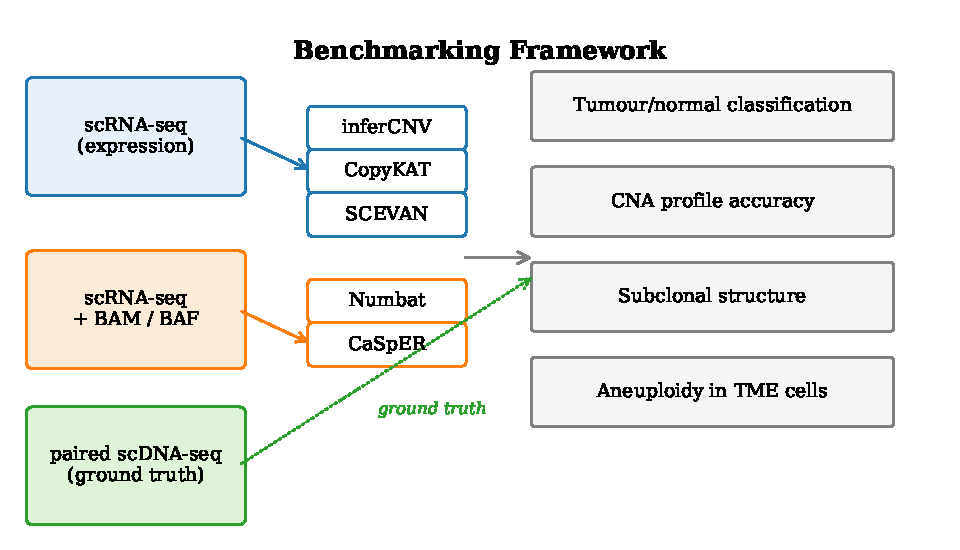
\includegraphics[width=0.9\textwidth]{figures/fig_workflow.pdf}
\caption{Overview of the benchmarking framework. Five scRNA-seq-based CNA
inference tools are evaluated in two methodological categories:
expression-only (inferCNV, CopyKAT, SCEVAN) and expression-plus-allele
(Numbat, CaSpER). Paired scDNA-seq from single-cell multi-omics datasets
serves as ground truth across four evaluation tasks: tumour/normal
classification, CNA profile accuracy, subclonal structure inference, and
aneuploidy detection in non-malignant cells.}
\label{fig:workflow}
\end{figure}

\subsection{Benchmarking framework and datasets}

We first consolidated a panel of paired scRNA-seq and scDNA-seq datasets in
which the same cell's transcriptome and genome are measured jointly
(Figure~\ref{fig:workflow}). Because such multi-omic experiments are still
uncommon, we prioritised breadth of tumour types over depth within a single
tumour, retaining eight CRC samples, two ALL samples, one glioma, one
neuroendocrine tumour, the NPC43 cell line, a HUVEC normal cell line, and a
gastric sample for cnLOH validation (Table~\ref{tab:datasets}). This coverage spans solid tumours,
hematopoietic malignancies, and cancer cell lines, exposing each tool to the
full range of CNA complexity, tumour purity, and cell-count regimes
encountered in practice.

The five tools evaluated --- inferCNV, CopyKAT, SCEVAN, Numbat, and CaSpER
--- fall into two complementary categories (Table~\ref{tab:tools}). Three
operate solely on the expression matrix; the remaining two (Numbat, CaSpER)
additionally ingest B-allele frequencies, which is informative for LOH but
requires access to raw BAM files. Performance was measured across four
applications: (i) tumour versus normal cell classification; (ii) accuracy of
inferred CNA events relative to scDNA-seq; (iii) tumour subclone inference;
and (iv) aneuploidy detection in non-malignant cells. The addition of
aneuploidy detection is motivated by accumulating evidence that CNAs also
occur in ostensibly non-malignant tissue~\cite{zhou2020singlecell} and may
influence cellular fitness.

\subsection{Distinguishing tumour from normal cells}

We first asked how well each tool separates tumour from normal cells based
on inferred CNA signal. Across the glioma, CRC, and neuroendocrine datasets,
Numbat performed best overall. Among the three expression-only tools,
CopyKAT was the strongest, consistent with its integrated Bayesian
segmentation and GMM-based normal-cell selection. SCEVAN exhibited poor
performance in samples with low tumour frequency (less than 40\%), such as
CRC11, CRC12, CRC16, and CRC15; its heavy reliance on TME gene signatures to
anchor the normal-cell reference appears to break down when TME-like cells
outnumber tumour cells. InferCNV was reliable across most samples except
CRC02, where the majority of cells are tumours (approximately 88\%). In
CRC02, the copy number gains and losses in tumour cells were incorrectly
centred as the baseline by inferCNV, and normal cells were consequently
predicted to harbour the opposite CNA profile and mis-classified as tumour
cells. CaSpER made the same error in CRC02.

\begin{figure}[htbp]
\centering
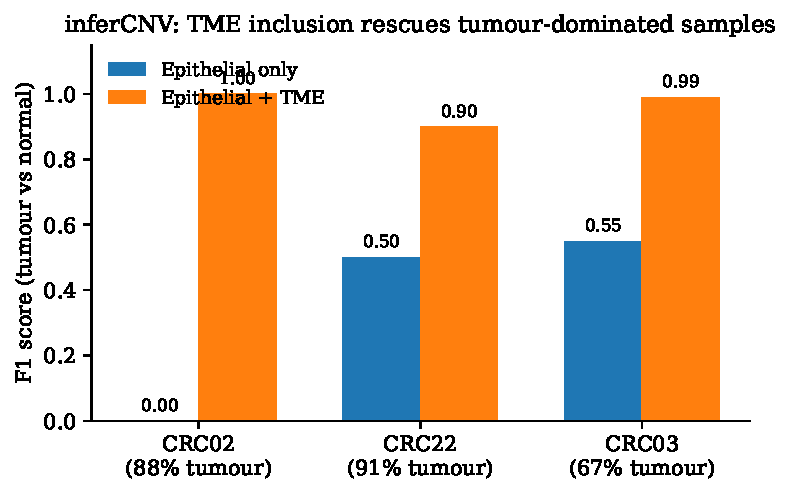
\includegraphics[width=0.7\textwidth]{figures/fig_tme_rescue.pdf}
\caption{Including tumour microenvironment (TME) cells rescues inferCNV F1
scores for tumour-normal classification in three CRC samples with high tumour
purity. For CRC02 (88\% tumour), CRC22 (91\%), and CRC03 (67\%),
epithelial-only F1 scores of 0, 0.5, and 0.55 rose to 1.0, 0.9, and 0.99
respectively when TME cells were added to the input.}
\label{fig:tme_rescue}
\end{figure}

The CRC02 finding suggested that incorrect centring is, at heart, a
reference-composition problem. We therefore tested whether explicitly adding
TME cells --- immune, endothelial, and fibroblast --- to the input would
shift the population-mean reference away from the tumour. Across the three
tools that do not require a reference (inferCNV, CopyKAT, SCEVAN), the
inclusion of TME cells significantly improved SCEVAN's tumour-normal
accuracy, consistent with its algorithmic reliance on TME gene signatures.
Although the overall improvement was less pronounced for inferCNV, certain
samples showed dramatic rescues: CRC02 (88\% tumour), CRC22 (91\% tumour),
and CRC03 (67\% tumour) moved from F1 = 0, 0.5, and 0.55 to F1 = 1.0, 0.9,
and 0.99 respectively (Figure~\ref{fig:tme_rescue}, Table~\ref{tab:tme}).
For CRC02, incorporating TME cells simultaneously improved tumour-normal
discrimination and recovered the correct CNA profile, including
amplifications on chr8 and chr20 and deletions on chr15. This rescue is
consistent with the hypothesis that a higher-purity sample starves inferCNV
of a neutral baseline: TME cells supply the missing baseline, and both the
classification step and the downstream CNA profile benefit. Supporting this
interpretation, inferCNV also performed very well on CRC15, where tumour
purity is exceptionally low (6\%) and the baseline problem does not arise.

\begin{table}[htbp]
\centering
\caption{Effect of TME inclusion on inferCNV F1 for tumour-normal
classification in tumour-dominated CRC samples.}
\label{tab:tme}
\small
\begin{tabular}{lccc}
\toprule
Sample & Tumour purity & F1 (epithelial only) & F1 (epithelial + TME) \\
\midrule
CRC02 & 88\% & 0    & 1.0  \\
CRC22 & 91\% & 0.5  & 0.9  \\
CRC03 & 67\% & 0.55 & 0.99 \\
\bottomrule
\end{tabular}
\end{table}

\begin{table}[htbp]
\centering
\caption{Statistical tests used per analysis, with significance codes
NS: $p > 0.05$; $*$: $p < 0.01$; $**$: $p < 0.001$; $***$: $p < 0.0001$.}
\label{tab:stats}
\small
\begin{tabular}{lll}
\toprule
Comparison & Test & Correction \\
\midrule
Epithelial vs epithelial + TME F1 (paired samples) & Paired Wilcoxon rank-sum & --- \\
F1 across tools at varying purity / depth / filter-pass & Kruskal--Wallis    & --- \\
One-pass vs two-pass inferCNV Pearson correlation    & Wilcoxon rank-sum (unpaired) & Benjamini--Hochberg \\
\bottomrule
\end{tabular}
\end{table}

To systematically probe how tumour purity shapes classification, we
generated a synthetic dataset spanning T:N ratios from 1:100 to 100:1 using
the largest glioma dataset, resampling each ratio 50 times. Numbat
consistently outperformed the other tools, even in extreme cases with very
low tumour purity. InferCNV exhibited opposite-calling between tumour and
normal cells when tumour purity was high, mirroring the CRC02 behaviour.
These results establish that CNAs inferred from expression alone are
fundamentally sensitive to the composition of the cell population that
defines the baseline.

We next asked how sequencing depth constrains accuracy by downsampling
samples to median 10K, 3K, and 1K UMIs per cell. The tumour-normal F1 for
all tools declined with depth, with Numbat showing the sharpest drop: its
dependence on allele counts, which are inherently rarer than expression
signals, appears to be the limiting factor. CopyKAT, in contrast, was
remarkably robust: even at 1K UMIs per cell it correctly distinguished
tumour from normal cells, although the CNA signal-to-noise ratio clearly
decreased. The apparent paradox of increasing SCEVAN F1 at low depth turned
out to be an artefact of aggressive cell filtering: lower-depth cells were
filtered out, which rectified the tool's bias toward assigning non-malignant
cells as malignant. Cell filtering is implemented in inferCNV, CopyKAT, and
SCEVAN but not in Numbat or CaSpER, and this accounts for much of the
cross-tool variability under depth stress.

Taken together, balanced tumour and normal ratios erase most between-tool
differences for the classification task, but imbalance or low depth exposes
real methodological weaknesses. When BAF is available, Numbat is the method
of choice; when only an expression matrix is available, or when sequencing
depth is shallow, CopyKAT is the safest option.

\subsection{Accuracy of inferred CNA profiles}

Having quantified tumour-normal classification, we turned to the accuracy of
the inferred CNA profiles themselves. Because reference-cell composition
strongly influences inferCNV centring, we first asked whether running
inferCNV in two-pass mode --- where normal cells predicted by a one-pass run
become the reference for a second run (Figure~\ref{fig:two_pass}) ---
improves the concordance between scRNA-seq and scDNA-seq CNA profiles. The
Pearson correlation between inferred and ground-truth CNA profiles increased
significantly in eight of nine cases. CopyKAT and SCEVAN already implement a
two-pass-like procedure internally, and introducing an external two-pass
wrapper made negligible difference to their output.

\begin{figure}[htbp]
\centering
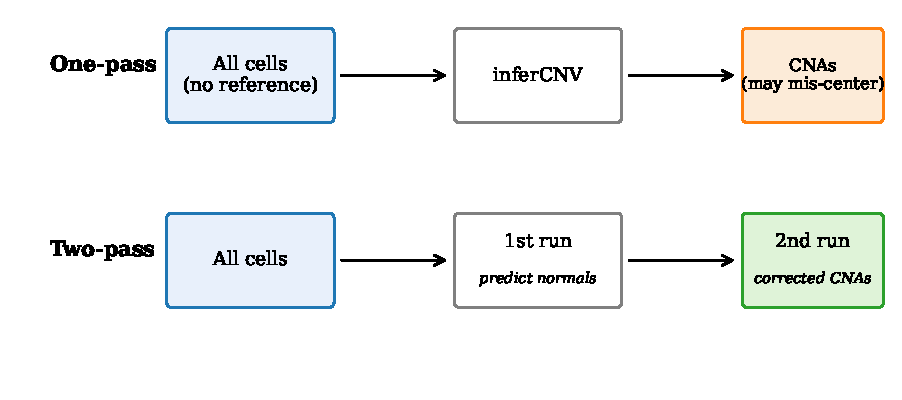
\includegraphics[width=0.9\textwidth]{figures/fig_two_pass.pdf}
\caption{One-pass versus two-pass inferCNV reference setting. In one-pass
mode (top) the whole cell population serves as its own reference, which can
mis-centre copy number profiles when tumour purity is high. In two-pass
mode (bottom) cells predicted as normal in the first run are used as the
reference for a second run, yielding corrected CNA profiles.}
\label{fig:two_pass}
\end{figure}

With every tool running in its best-performing configuration, no single tool
dominated the CNA accuracy comparison across samples. Numbat and CaSpER
produce integer CNA calls that are easier to interpret and appear cleaner,
whereas inferCNV, CopyKAT, and SCEVAN produce continuous CNA values. All
five tools performed well on samples with sufficient numbers of both tumour
and normal cells --- for example, glioma, CRC13, CRC11, and CRC12 --- where
the baseline can be reliably estimated. In imbalanced samples such as
CRC02, CRC22, and CRC15, per-sample accuracy dropped considerably across
all tools. CRC03 produced a striking asymmetry: Numbat correctly assigned
the tumour cells but recovered only a small fraction of the deletions in the
high-CNA-burden tumour population, yielding low Pearson correlation with
scDNA-seq. This decoupling between classification and profile accuracy is
itself diagnostic: a tool that correctly separates tumour cells can still
mis-characterise the profile shape.

On the two ALL samples, we could only evaluate inferCNV, CopyKAT, and SCEVAN
because raw FASTQ data were unavailable for allele calling. CopyKAT gave the
best performance on ALL, but both CopyKAT and SCEVAN produced noticeable
false-positive CNA signals. On cancer cell lines profiled in isolation, all
tools except Numbat performed poorly; the inclusion of normal cells
(HUVEC) rescued the four expression-based tools but not Numbat. The
dependence on haplotype phasing combined with a small number of homogeneous
cells appears to be a harder operating regime for Numbat than for the
expression-based tools.

Clonal breakpoint detection was evaluated against pseudo-bulk scDNA-seq
calls (circular binary segmentation plus MergeLevels) with a 200\,kb window
for matching. Considerable variation in segment counts was observed across
tools: Numbat and CaSpER reported tens to hundreds of segments per cell,
whereas CopyKAT and SCEVAN reported thousands, which clearly exceeds the
expected number of chromosomal breakpoints in cancer. Because CopyKAT and
CaSpER do not implement a clonal breakpoint function, we focused breakpoint
evaluation on inferCNV, SCEVAN, and Numbat. SCEVAN achieved the best F1
score and sensitivity, whereas inferCNV was the most precise. Both inferCNV
and Numbat detected far fewer breakpoints than SCEVAN and the ground truth
from scDNA-seq. On chromosome 10, for instance, SCEVAN resolved two adjacent
deletions as separate breakpoints, while inferCNV and Numbat merged them
into a single event. On chromosome 14, inferCNV and Numbat missed a
breakpoint that SCEVAN detected. Numbat also occasionally reported
false-positive CNAs, as on chromosome 1.

\begin{figure}[htbp]
\centering
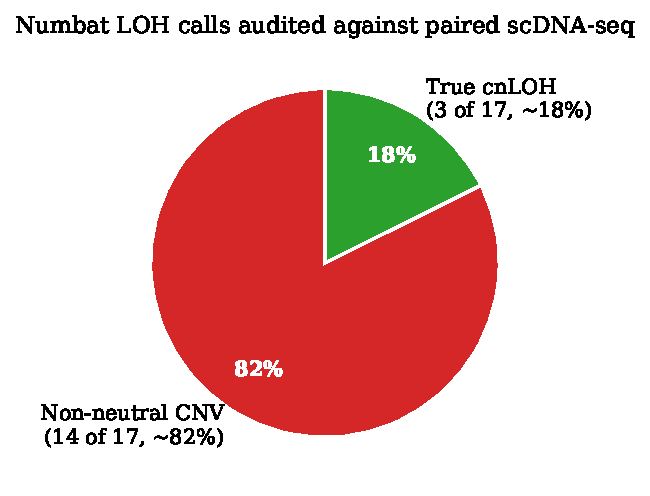
\includegraphics[width=0.55\textwidth]{figures/fig_loh_breakdown.pdf}
\caption{Audit of Numbat LOH calls against paired scDNA-seq allele-specific
copy number states. Of 17 LOH events reported by Numbat across multiple
samples, 14 ($\sim$82\%) were in fact non-neutral CNV events (amplifications
or deletions), while 3 corresponded to genuine copy-number-neutral LOH
(cnLOH).}
\label{fig:loh_breakdown}
\end{figure}

Because both Numbat and CaSpER can call LOH by combining expression with
allele information, we audited their LOH outputs against paired scDNA-seq.
CaSpER produced too many obvious false positives in both malignant and
non-malignant cells and was not evaluated further. Numbat reported 17 LOH
events across the cohort. When we then inspected the true CNV status of
these regions using Sequenza~\cite{favero2015sequenza} on merged pseudo-bulk
scDNA-seq BAM files, 14 of 17 events ($\sim$82\%) turned out to be
non-neutral CNV events --- amplifications or deletions --- rather than true
copy-number-neutral LOH (Figure~\ref{fig:loh_breakdown}). For instance, in
CRC13 Numbat identified chr8q as an LOH event, but scDNA-seq revealed a
CNV amplification on 8q driven by a copy-number gain on the A allele while
the B allele remained unchanged. Nevertheless, Numbat showed high
sensitivity for genuine cnLOH: three regions on chr5q, chr12q, and chr17p in
CRC13 were confirmed as cnLOH by Sequenza AB allele states (B-allele copy
number zero at neutral total copy). The chr17p cnLOH caused loss of
heterozygosity of \emph{TP53}, consistent with its role as a driver event in
cancer evolution. In an independent validation on a gastric sample (GX109)
with four annotated cnLOH events from a prior study, Numbat correctly
recovered all four events with no false positives.

In summary, no single tool uniformly dominated CNA profile accuracy. SCEVAN
delivered the best F1 for breakpoint detection, and Numbat showed high
sensitivity for cnLOH; but Numbat's LOH output requires independent
validation because most of its calls were non-neutral CNV events driven by
the resolution limits of its genotype modelling.

\subsection{Subclonal structure inference}

Intra-tumoural heterogeneity, driven by emerging subclones with distinct
mutations and CNAs~\cite{mcgranahan2017clonal}, is a central question for
scRNA-seq-based CNA analysis. We evaluated subclonal inference on samples
with at least 10 tumour cells --- glioma and seven CRC samples. Optimal
cluster counts selected by average silhouette scores were typically $k = 2$
for CRC samples; when more than two subclones were predicted, we merged
clusters by profile similarity. Upon manual inspection, two CRC samples ---
CRC03 and CRC11 --- carried two sizeable subclones.

For glioma, only Numbat correctly assigned the smaller C1 subclone as tumour
cells (14 of 15 cells correctly classified); the other tools either
mis-classified C1 as normal or failed to resolve the subclones at all. We
therefore tested subclone inference on glioma only with Numbat: the
inferred subclone structure was largely consistent with the scDNA-seq ground
truth. In CRC03, only inferCNV failed to resolve the two subclones,
incorrectly classifying the C1 subclone as normal; adding TME cells rescued
the subclonal structure along with the classification. In CRC11, where all
tools correctly classified tumour cells, every tool achieved ARI $>$ 0.8.
In one extreme case within CRC12, a subclone consisted of a single cell, and
only inferCNV and SCEVAN detected that single-cell subclone. These results
underline that the prerequisite for accurate subclonal inference is accurate
tumour-normal classification: once cells are correctly labelled as tumour,
hierarchical clustering of their CNA profiles tends to recover the subclones
faithfully across tools.

Building on the robustness of subclone assignment once tumour-normal
labels are correct, we next asked the opposite question: can these tools
resolve the much rarer and lower-burden CNA events that occur in
non-malignant cells?

\subsection{Aneuploidy detection in non-malignant cells}

Accumulating evidence indicates that non-malignant cells can harbour CNAs
that influence cellular fitness~\cite{zhou2020singlecell}. We therefore
asked whether these tools, which are tuned for the complex CNA landscapes
of tumours, could detect whole-chromosome aneuploidies in normal cell types.
We selected four cell types with known autosomal aneuploidy events ---
fibroblasts, T cells, B cells, and endothelial cells --- and evaluated
sensitivity, specificity, and F1 score. All tools performed poorly on this
task, reflecting two compounding factors. First, CNA complexity in
non-malignant cells is much lower than in tumour cells, typically limited to
single whole-chromosome gains or losses, which offers a much weaker
expression-level signal for any of the tools to lock onto. Second, both UMI
counts and gene counts per cell are significantly lower in non-malignant
cells than in matched malignant cells, further degrading the
signal-to-noise ratio. Detecting low-burden aneuploidy in non-malignant
cells therefore remains an unmet computational need.

\subsection{Computational performance}

To compare computational cost, we measured CPU time on a single-core setting
on a high-performance computing platform. CopyKAT and SCEVAN were the
fastest, inferCNV and CaSpER moderate, and Numbat the slowest. Runtime
increased only gradually with dataset size but remained acceptable for every
tool on our cohort. The dominant cost for Numbat and CaSpER is the
per-sample calculation of BAF from BAM files, which can be trivially
parallelised across samples. A laptop is adequate for datasets below 1000
cells, but cases with several thousand cells are best analysed on a server
or HPC platform, particularly for Numbat and inferCNV.

\section{Discussion}

This benchmark provides the first independent head-to-head comparison of the
five most widely used scRNA-seq-based CNA inference tools against paired
scDNA-seq ground truth. Across tumour-normal classification, CNA profile
accuracy, subclonal structure inference, and aneuploidy in non-malignant
cells, Numbat was the top overall performer, as might be expected from its
haplotype-aware HMM architecture~\cite{gao2023numbat}. When only an
expression matrix is available, or when sequencing depth is shallow,
CopyKAT~\cite{gao2021copykat} emerged as the most reliable choice; its
robustness down to 1K UMIs per cell is particularly valuable for low-depth
or retrospective datasets. SCEVAN~\cite{defalco2023scevan} achieved the best
F1 score for clonal breakpoint detection, and together with the
methodological summary in Table~\ref{tab:tools} these findings supply a
practical decision tree for tool selection.

A recurring theme of our results is that expression-based methods are more
susceptible to biases in reference-cell composition than their
allele-augmented counterparts. Without a reference setting, inferCNV relies
on the input population to estimate a neutral baseline, and when tumour
purity is high, genuine CNA signals can be absorbed into the baseline and
the resulting centring error propagates to normal cells. Concretely, CRC02
(88\% tumour) moved from F1 = 0 to F1 = 1.0 when TME cells were added
(Figure~\ref{fig:tme_rescue}); similar rescues occurred for CRC22 and CRC03.
Conversely, SCEVAN tended to misassign non-malignant cells as malignant when
tumour purity was low, and the same intervention --- including TME cells
--- improved performance for the complementary reason: it provided the TME
gene signatures that SCEVAN's internal normal-cell detection expects.
Reference-cell composition is therefore not a peripheral implementation
detail but a first-order factor in every expression-based pipeline.

The LOH audit highlights a subtle cost of Numbat's otherwise strong
allele-aware design. While Numbat is highly sensitive to genuine cnLOH ---
it recovered all four previously annotated cnLOH events in the gastric
sample GX109 without false positives, and validated chr5q, chr12q, and
chr17p cnLOHs in CRC13 using Sequenza~\cite{favero2015sequenza} --- it
over-calls LOH globally: 14 of 17 events in our cohort ($\sim$82\%) were
actually CNV amplifications or deletions with one allele lost
(Figure~\ref{fig:loh_breakdown}). The driver is a resolution gap in
Numbat's genotype model between the (1,0) genotype (single-copy deletion
with LOH) and the (2,0) genotype (copy-number-neutral LOH), and the
asymmetric prior that disfavours highly imbalanced gain genotypes such as
(3,1). Users of Numbat should treat its LOH output as a screening call and
verify neutral copy-number state with independent approaches before drawing
biological conclusions, especially when interpreting tumour-suppressor loci
such as \emph{TP53}.

Complexity and modality of CNAs also shape how each tool behaves. All tools
performed better on solid tumours than on hematopoietic cancers or on cell
lines, consistent with the lower CNA complexity and lower chromosomal
heterogeneity of hematopoietic malignancies. This observation suggests that
tools tuned on solid tumours may need recalibration for leukaemias, and that
cell-line benchmarks with accompanying normal cells (as in our HUVEC
control) are essential to avoid misleading performance estimates. The
broadly poor performance on aneuploidy detection in non-malignant cells
underscores a methodological gap: existing tools are designed for the
high-burden CNA landscapes of tumours, not for the single-chromosome events
typical of benign tissue, and the lower UMI counts in non-malignant cells
compound the signal-to-noise problem. Developing scRNA-seq-based methods
capable of detecting low-burden aneuploidy in benign tissue is a concrete
future direction that would extend these analyses beyond cancer and into
tissue biology, immunity, and development.

Sequencing depth is the other systematic factor we examined, and its effect
is not uniform. Numbat's performance degraded significantly below 10K UMIs
per cell, reflecting the scarcity of informative allele counts at low
depth. InferCNV and especially CopyKAT were more forgiving, with CopyKAT
maintaining correct tumour-normal classification at median 1K UMIs per
cell. The apparent F1 improvement of SCEVAN at low depth was attributable to
aggressive cell filtering rather than better inference, which is easy to
misinterpret. Study design should therefore match tool choice to
anticipated depth: for targeted deep sequencing of selected samples, Numbat
is powerful; for broad, shallow profiling, CopyKAT combined with a second
tool is safer.

Several limitations deserve explicit acknowledgement. First, paired
single-cell multi-omics datasets remain scarce, which caps the sample sizes
in each comparison and limits our ability to evaluate very large datasets
of the scale now routine on droplet platforms. Second, small cell counts
limit subclonal structure evaluation, particularly for rare subclones such
as the single-cell subclone in CRC12. Third, parameter settings play a
first-order role, and the optimal settings can be both sample-specific and
task-specific; we observed, for instance, that a smaller Numbat
\texttt{gamma} parameter improved tumour-normal separation but compromised
breakpoint detection. We therefore recommend that practitioners combine
literature guidance with a small parameter sweep on representative samples.

Given that no single tool excelled in every task, we recommend running
analyses with at least two complementary tools. When raw BAM data are
available, we suggest combining Numbat~\cite{gao2023numbat} with either
SCEVAN~\cite{defalco2023scevan} or inferCNV~\cite{tickle2019infercnv};
this pairing combines Numbat's allele-aware precision with SCEVAN's
breakpoint sensitivity or inferCNV's precision advantage. When only an
expression matrix is available, we recommend pairing
CopyKAT~\cite{gao2021copykat} with either SCEVAN or inferCNV. The broader
implication is that many lessons learned here --- the primacy of reference
composition, the depth-sensitivity of allele-augmented methods, and the
caution needed for LOH interpretation --- carry directly into emerging
spatial transcriptomics pipelines, which face the same inference challenge
with the additional complication of spot-level rather than cell-level
resolution.

In summary, this study offers a much-needed independent comparison of
scRNA-seq-based CNA inference tools and supplies concrete, data-grounded
guidance for their use. By tying each recommendation to a paired-omics
ground truth rather than to a self-reported internal benchmark, we give
researchers a firmer basis for choosing among tools and for interpreting
their output under real-world conditions of varying tumour purity,
sequencing depth, and reference availability. Our hope is that the pairings
and parameter notes above accelerate reliable CNA analysis in the
increasingly large and diverse scRNA-seq datasets now being produced, and
that the gaps identified --- particularly low-burden aneuploidy detection
and LOH precision --- motivate the next generation of methods.

\bibliography{references}

\end{document}
